% SETUP
\documentclass[11pt]{article}
\linespread{1.25}
\usepackage[utf8]{inputenc}
\usepackage{graphicx, amsmath, array, graphics, amssymb, epsfig, psfrag, geometry, alltt, subfiles, blindtext, float}
\usepackage[dvipsnames]{xcolor}
\usepackage[export]{adjustbox}
\usepackage{fancyhdr}
\usepackage{array}
\usepackage{hyperref}
\geometry{a4paper, top = 20mm, bottom = 20mm, left = 15mm, right = 15mm}

% Headers
\pagestyle{fancy}
\fancyhf{}
\chead{ELEN90066 Embedded Systems Design - Workshop 4 Prelab}
\cfoot{\thepage}

\begin{document}

% Title
\begin{center}
\textbf{\Large{Workshop 4 Prelab}}\\
YiLin Inez Zheng [702279], \\
Workshop: Monday 3:15pm - 6:15pm, Due: 02/09/19  
\end{center}

\section{Section 6.4.2}
\subsection{Kobuki Equipment exercises form 1.5.3}
\begin{enumerate}
    \item %1
    The Kobuki has on the bottom: 3 Docking IR sensors (left, right, centre), 3 Bump sensors (left, right, centre), 3 Cliff sensors (left, right, centre) and 2 Wheel drop sensors (left, right).\\ 
    \underline{This totals to 11 sensors on the bottom.}
    \item %2
    Bytestream: Header 1 - \texttt{0xAA}, Header 0 - \texttt{0x55}, Length - \texttt{0x06}, Payload - see below, Checksum - \texttt{0x00}\\
    \textcolor{blue}{Payload}: Header - \texttt{0x01}, Length - \texttt{0x04}, Data (speed) - \texttt{0x012C}, Data (radius) - \texttt{0x0000}\\
    Serialised bytestream: \texttt{0xAA5506\textcolor{blue}{01042C010000}00}
    \item %3
    Bytestream: Header 1 - \texttt{0xAA}, Header 0 - \texttt{0x55}, Length - \texttt{0x0C}, Payload - see below, Checksum - \texttt{0x00}\\
    \textcolor{blue}{Subpayload - Left turn}: Header - \texttt{0x01}, Length - \texttt{0x04}, Data (speed) - \texttt{0x00FA}, Data (radius) - \texttt{0x0001}\\
    \textcolor{orange}{Subpayload - Right turn}: Header - \texttt{0x01}, Length - \texttt{0x04}, Data (speed) - \texttt{0x012C}, Data (radius) - \texttt{0x1111}\\
    Serialised bytestream: \texttt{0xAA550C\textcolor{blue}{01040100FA00}\textcolor{orange}{01042C011111}00}\\
    Also expressing -1 from the right turn radius as 0x1111 using twos complement.
    \item %4
    Bytestream: Header 1 - \texttt{0xAA}, Header 0 - \texttt{0x55}, Length - \texttt{0x11}, Payload - see below, Checksum - \texttt{0x00}\\
    \textcolor{blue}{Payload}: Header - \texttt{0x01}, Size - \texttt{0x0F}, Bumper (right, centre) - \texttt{0x03}, Button 2 - \texttt{0x04}\\
    Serialised bytestream: \texttt{0xAA5511\textcolor{blue}{xxxx03xxxxxxxxxxxxxx04xxxxxxxx}00}
\end{enumerate}

\subsection{State Machine}
\begin{figure}[H]
    \centering
    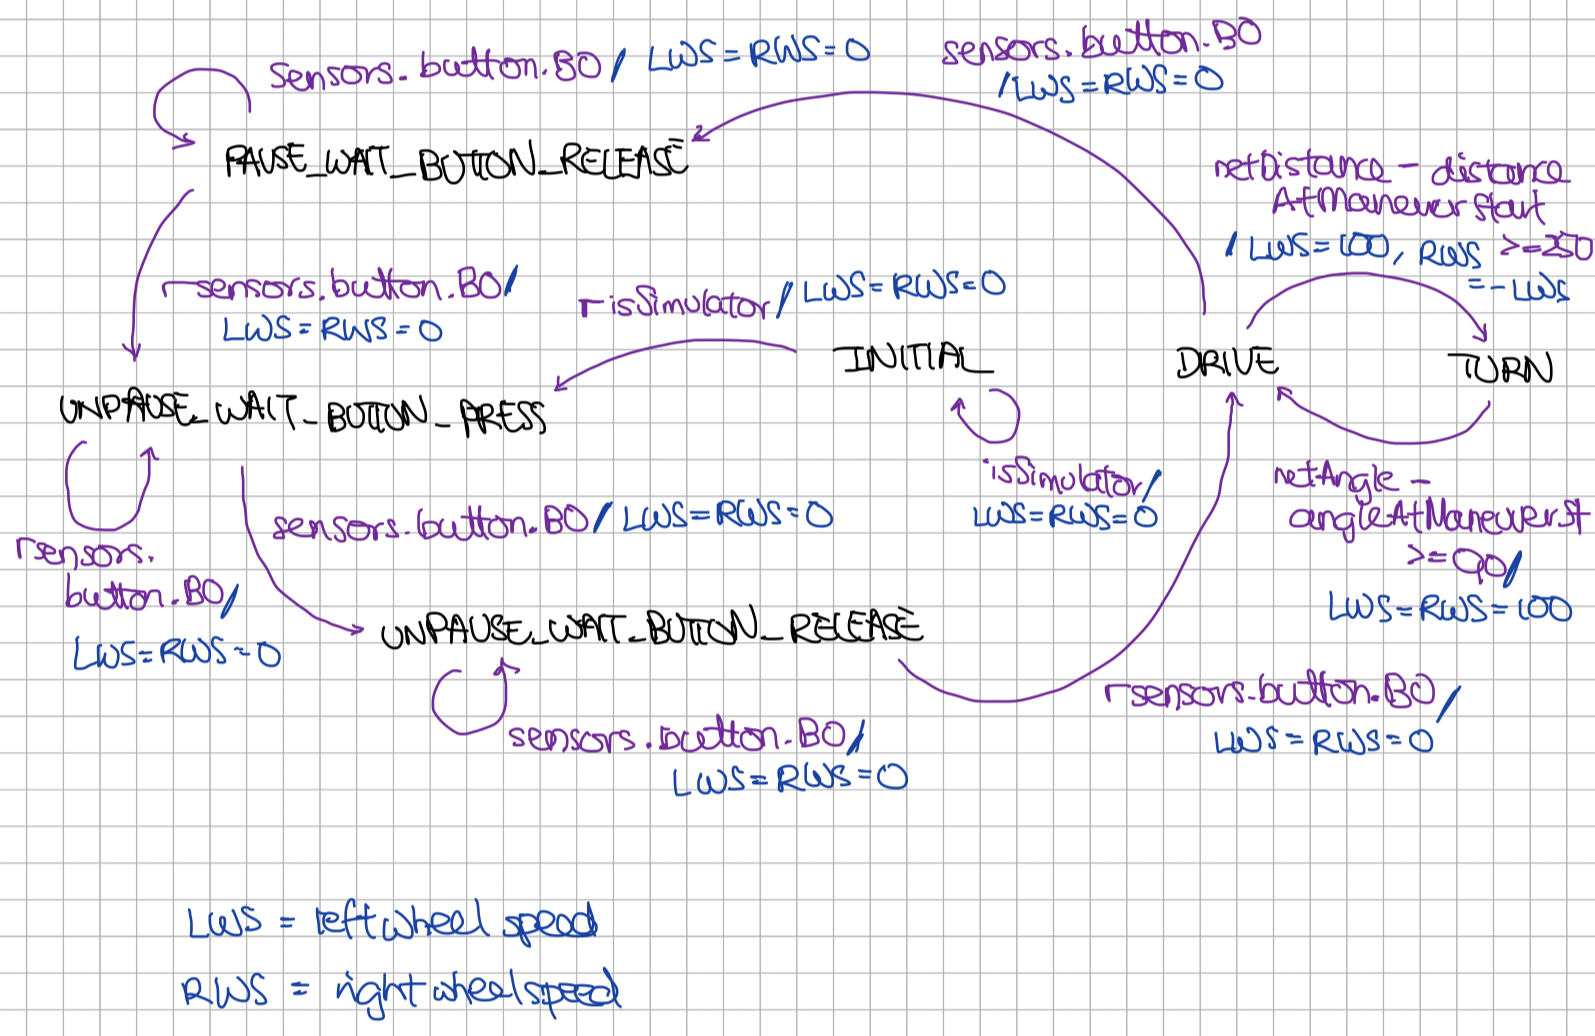
\includegraphics[scale=0.26]{FSM.jpeg}
    \caption{Sketch of the FSM from \texttt{KobukiNavigationStateChart.c}}
    \label{fig:FSM}
\end{figure}
%\textit{Notes:}\\
%AI0: Wheel speed right (0V - full speed backward, 3.3V - full speed forward)\\
%AI1: Wheel speed left (0V - full speed backward, 3.3V - full speed forward)\\
%AI0-3: 4 x Analog input (12bit ADC: 0 - 4095, 0 - 3.3V)

\section{Section 6.5.2}
\subsection*{Kobuki Equipment Exercises}
\begin{enumerate}
    \item %1 
    \begin{enumerate}
        \item %a
        The Kobuki protocol periodically sends feedback at a rate of 50Hz - this is a time based interrupt. The \texttt{main.c} polls sensors for data.
        \item %b
        Delay the execution and polling by 5 seconds. Set \texttt{msDelay = 5000} in \texttt{main.c}.
    \end{enumerate}
\end{enumerate}
\end{document}